%%% Formal Model-based Validation for Tally Systems
% VoteID version - March 2013

\documentclass[runningheads,a4paper]{llncs}

\usepackage{eurosym}
\usepackage{longtable}
\usepackage{tabularx}
\usepackage{epsfig}
\usepackage{amsmath}
\usepackage{amsfonts}
\usepackage{eucal}
\usepackage{float}
\usepackage{listings}
\usepackage{ntheorem}
\usepackage{pseudocode}
\usepackage[pdftex,bookmarks=false,
            plainpages=false,naturalnames=true,
            colorlinks=true,pdfstartview=FitV,
            linkcolor=blue,citecolor=blue,urlcolor=blue, 
            pdfauthor="Mystery Zero and Mystery One"]{hyperref}
\usepackage{xspace}

\newcommand{\eg}{e.g.,\xspace}
\newcommand{\ie}{i.e.,\xspace}
\newcommand{\etc}{etc.\xspace}
\newcommand{\votail}{V\'{o}t\'{a}il\xspace} 
\newcommand{\eireann}{\'{E}ireann}
\newcommand{\dail}{D\'{a}il\xspace}
\newcommand{\outcome}{\ensuremath{\mathcal{O}}\xspace}
\newcommand{\scenario}{\ensuremath{\mathcal{S}}\xspace}
\newcommand{\ballots}{\ensuremath{\mathcal{B}}\xspace}
\newcommand{\ballotspec}{\ensuremath{\Phi}\xspace}
\newcommand{\config}{\ensuremath{\ballots \vdash_\scenario \outcome}\xspace}
\newcommand{\candidates}{\ensuremath{\mathcal{C}}\xspace}
\newcommand{\election}{\ensuremath{\mathcal{E}}\xspace}
\newcommand{\winners}{\ensuremath{\mathcal{W}}\xspace}
\newcommand{\losers}{\ensuremath{\mathcal{L}}\xspace}
\newcommand{\ballotone}[1]{\ensuremath{\boxed{#1}}}
\newcommand{\ballottwo}[2]{\ensuremath{\boxed{#1}\boxed{#2}}}
\newcommand{\ballotthree}[3]{\ensuremath{\boxed{#1}\boxed{#2}\boxed{#3}}}
\newcommand{\ballotfour}[4]{\ensuremath{\boxed{#1}\boxed{#2}\boxed{#3}\boxed{#4}}}
\newcommand{\winner}{\ensuremath{\mathbb{W}}}
\newcommand{\earlyloser}{\ensuremath{\mathbb{E}}}
\newcommand{\earlyloserNT}{\ensuremath{\mathbb{F}}}
\newcommand{\loser}{\ensuremath{\mathbb{L}}}
\newcommand{\quota}{\ensuremath{\mathbb{Q}}}
\newcommand{\belowthreshold}{\ensuremath{\mathbb{S}}}
\newcommand{\earlybelowthreshold}{\ensuremath{\mathbb{D}}}
\newcommand{\earlybelowthresholdNT}{\ensuremath{\mathbb{U}}}
\newcommand{\quotawinnernontransferable}{\ensuremath{\mathbb{X}}}
\newcommand{\winnernontransferable}{\ensuremath{\mathbb{N}}}
\newcommand{\abovequotawinner}{\ensuremath{\mathbb{A}}}
\newcommand{\highwinner}{\ensuremath{\mathbb{H}}}
\newcommand{\surpluswinner}{\ensuremath{\mathbb{T}}}
\newcommand{\tiebreak}[1]{\ensuremath{\underline{#1}}}
\newcommand{\first}{$1^{st}$\xspace}
\newcommand{\second}{$2^{nd}$\xspace}
\newcommand{\third}{$3^{rd}$\xspace}

\newtheorem{Lemma}{Lemma}
\newtheorem{Definition}{Definition}
\newtheorem{Theorem}{Theroem}

\newcommand{\myhref}[2]{\ifpdf\htmladdnormallink{#2}{#1}\else\htmladdnormallinkfoot{#2}{#1}\fi}

\begin{document}

% don't want date printed
\date{}

% make title bold and 14 pt font (Latex default is non-bold, 16 pt)
\title{Formal Model-based Validation\\ for Tally Systems}
%\subtitle{Using the Alloy Model Finder to Derive Test Cases for PR-STV Elections}

\author{Mystery Author Zero\inst{1} and Mystery Author One\inst{2}}
%\author{Dermot Cochran\inst{1} and Joseph R. Kiniry\inst{2}}

\institute{Mystery Workplace Zero \and
Mystery Workplace One}

% \institute{Siemens A/S, Ballerup, Denmark\\
% \email{dermot.cochran@siemens.com} \and
% Technical University of Denmark, Lyngby, Denmark\\
% \email{jkin@imm.dtu.dk}}

\maketitle

% Use the following at camera-ready time to suppress page numbers.
% Comment it out when you first submit the paper for review.
%\thispagestyle{empty}

\begin{abstract}
  Existing commercial and open source e-voting systems have
  horrifically poor testing frameworks.  Most tally systems, for
  example, are tested by re-running all past elections and seeing if
  the new system gives the same answer as an older, perhaps erroneous,
  system did.  This amounts to a few dozen system tests and,
  typically, few-to-no unit tests.  These systems are used today in a
  dozen countries to determine the outcome of national elections.
  This state-of-affairs cannot continue because it calls into question
  the legitimacy of elections in major European and North American
  democracies.

  In this work, the ballot counting process for one of the most
  complex electoral schemes used in the world, Proportional
  Representation by Single Transferable Vote (PR-STV), is mechanically
  formally modeled.  The purpose of such a formalization is to
  generate, using an algorithm of our design, a complete set of
  non-isomorphic test cases \emph{per electoral scheme}, once and for
  all.  Using such a system test suite, any digital election
  technology (proprietary or open source) can be rigorously evaluated
  for correctness.  Doing so will vastly improve the confidence
  experts have---and can only improve the level of trust citizens
  have---in these digital elections systems.
\end{abstract}

%=====================================================================
\section{Introduction}

The electoral process consists of various different stages, from voter
registration, through vote casting and tallying, to the final
declaration of results.  Some, but not all, aspects of the election
process are apparently suitable for automation.  For example, voter
registration records can be stored in computer databases, and ballot
counting can be done by machine.
% In Denmark, the final result of the election is
% calculated by a computer in the Danish Ministry of the Interior.
However, many attempts to introduce electronic counting of ballots
have failed, or at least received much criticism, due to software and
hardware errors, \emph{including potential counting errors}, many of
which are avoided through the appropriate use of formal methods and
careful testing.  The security aspects of elections, including voter
privacy and election integrity, are an important concern, but are
beyond the scope of this paper.

One of the potential advantages from automation is the \emph{accuracy
  of vote counting}, so it is important to be able to prove that
software can actually count ballots more accurately than the manual,
labor-intensive process of counting paper ballots by hand, especially
for complex voting schemes.  Measured error rates for manual tallying
of even simple electoral schemes range from around 0.5\% to 1.5\%.
Mechanical tallying of (well-formed, unadulterated) digital ballots
must have an error rate of 0\%.

In this paper we focus mainly on the Irish voting scheme, as a case
study, as it is one of the most complex electoral schemes in the
world.  By virtue of the design of this scheme and the manner in which
we formalize it, we also mechanize two other popular voting schemes.
We use the Alloy model finder~\cite{jackson2002alloy} to describe the
elections in terms of scenarios, consisting of equivalence classes of
possible outcomes for each candidate in the election, where each
outcome represents one branch through the algorithm.  We show how test
data is generated from a first-order logic representation of the
counting algorithm using the Alloy model finder.  This algorithm
guarantees that we find the smallest number of ballots needed to test
each scenario.

% --------------------------------------------------------------
\subsection{The Irish Voting Scheme}

The Republic of Ireland uses Proportional Representation by Single
Transferable Vote (PR-STV) for its national, local and European
elections.  Ireland uses Instant Runoff Voting (IRV) for its
presidential elections and for by-elections to fill casual vacancies
in \dail \eireann.  PR-STV is a multi-seat ranked choice voting system
in which each voter ranks the candidates from first to last
preference.  IRV is PR-STV with just one remaining seat.

Manual recounts are often called for closely contested seats, as the
results often vary slightly, indicating small errors in the manual
process of counting votes.  Paper-based voting with counting by hand
is popular in Ireland, and recent attempts at automation were
frustrated by subtle logic errors in the ballot counting
software~\cite{Coyle2004}.  The potential for logic errors exist, in
part, due to the complexities and idiosyncrasies with regard to tie
breaking, especially involving the rounding up or down of vote
transfers.

There has been some desire in Ireland to simplify matters.  Referenda
to introduce plurality (first past the post, where the candidate with
the most votes is the winner, as is used in the U.S.A. and the U.K.)
voting were rejected twice by the Irish electorate, once in 1959 and
again in 1968~\cite{sinnott1995irish}.  Since then, there have been no
further legislative proposals to change the voting scheme used in
Ireland.

The following are selected quotes from the Irish Commission on
Electronic Voting (CEV) report on the previous electronic voting
system used in Ireland (emphasis added)~\cite{CEV00}:
\begin{quote}
  \begin{itemize}    
  \item Design weaknesses, including \emph{an error in the
      implementation of the count rules that could compromise the
      accuracy of an election}, have been identified and these have
    reduced the Commission's confidence in this software.

  \item The achievement of the full potential of the chosen system in
    terms of secrecy and accuracy depends upon a number of software
    and hardware modifications, both major and minor, and more
    significantly, is dependent on the \emph{reliability of its software
    being adequately proven}.

  \item Taking account of the ease and relative cost of making some of
    these modifications, the potential advantages of the chosen
    system, once modified in accordance with the Commission's
    recommendations, can make it a \emph{viable alternative to the existing
    paper system in terms of secrecy and accuracy}.
  \end{itemize}
\end{quote}

Thus, Ireland wishes to keep its current complicated voting scheme, is
critical of the existing attempts to implement that scheme in
e-voting, but keeps the door slightly ajar for the introduction of
e-voting in the future.

% --------------------------------------------------------------
\subsection{Proportional Representation by Single Transferable Vote}

Proportional Representation by Single Transferable Vote (PR-STV)
achieves proportional representation in multi-winner elections, and
reduces to IRV for single-winner elections.

The following flowchart outlines the algorithm used for counting
preferences ballots by PR-STV.  A quota of preferences is chosen so
that at most $N-1$ candidates can reach the quota, where $N$ is the
number of seats to be filled.  A \emph{threshold} number or percentage
of votes is introduced to discourage unserious candidates---to be on a
ballot a candidate must put down a non-trivial deposit (say,
\euro1,000) and, if the number of vote for them does not reach the
threshold, they lose their deposit.  The threshold is always less than
the quota.  The surplus for a candidate is the number of votes in
excess of the quota.

\begin{center}
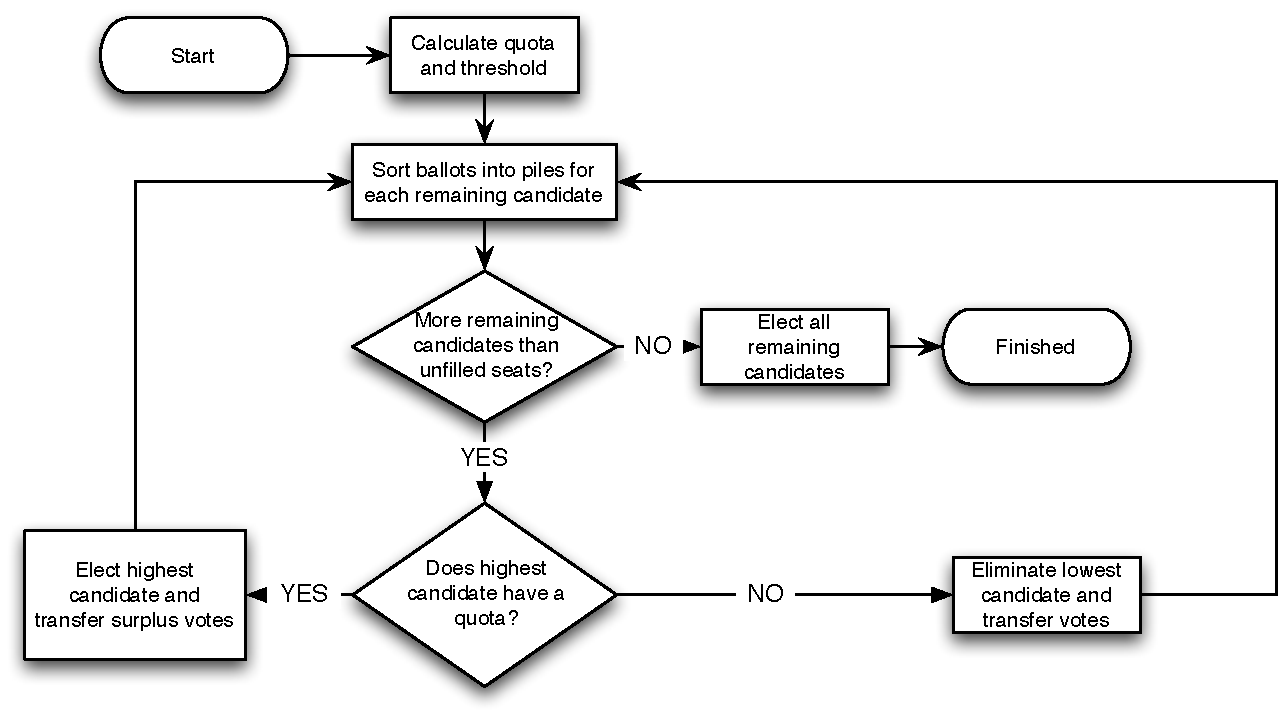
\includegraphics[width=110mm]{Process.pdf}
\end{center}

% --------------------------------------------------------------
\subsection{\votail}

\emph{\votail} is an open source Java implementation of Irish
Proportional Representation by Single Transferable Vote (PR-STV). Its
functional requirements, derived from Irish electoral law, were
formally specified using the Business Object Notation (BON) and
refined to a model-based Java Modeling Language (JML) specification.
While Normal and Extended Static Checking (ESC) were used to help
verify and validate the correctness of the software, the system was
not rigorously validated using system testing when it was first
developed.  Consequently, this new research enables us to rigorously
validate this (lightly, formally) verified tally system, further
increasing ones confidence in the system's correctness.

% --------------------------------------------------------------
\subsection{Related Work}

Related work in this area is thin in peer-reviewed publication venues,
as few groups in the world work on applying software engineering to
electionic election systems.  Some industrial and governmental work
exists, but much that we are aware of is either under NDA or is
word-of-mouth summaries of development practices at commercial firms.

\subsubsection{Academic Work}

Meagher wrote a Z and B specification (both are traditional formal
methods with tool support~\cite{Wing90}) for election to the board of
Waterford Institute of Technology, which uses a variant of the Irish
PR-STV system~\cite{Meagher01}.  Kj\"{o}lbro used a similar
methodology for specification and implementation of the Danish Voting
System~\cite{Kjolbro11}.  Neither system has been rigorously
validated through unit or system testing.

We are also aware of some unpublished work relating to a formalization
of PR-STV in $\lambda$-Prolog by Lee Naish.  It is our understanding
that this system was verified but not validated.

Researchers at the Radboud University Nijmegen attempted to test two
closed-source binaries implementing Scotland's tally system to ensure
its compliance with the WIG-rule~\cite{Scotland}.  To do so they did a
clean-room implementation of the Scottish STV system in the purely
functional programming language CLEAN and then compared nearly 6,000
hand-written and automatically generated test runs between all three
implementations~\cite{KoopmanEtAl07,KoopmanPlasmeijer11}.  It is
perhaps surprising that they found a number of errors in the
commercial implementations, given the ad hoc nature of their testing.

Researchers at the University College Dublin performed a similar
exercise on behalf of the aforemented CEV to test the closed source
``PowerVote'' tally system.  Their clean-room implementation was run
in parallel to the closed source binary on a network of workstations
for over one month on millions of randomly generated elections.  Using
this completely ad hoc technique they too found correctness errors in
the closed source tally system.

Also of interest is a protocol for the tallying of encrypted STV
ballots~\cite{TeagueEtAl08} and other work verifying properties of
voting protocols (e.g., several papers by Delaune and colleagues), but
none of this work focuses on rigorously developed or validated tally
systems.

All of these systems, even those that are semi-rigorously validated
(like those from Nijmegen), and \emph{especially} all of those that
are formally verified benefit from this new work.  The latter is true
since formally verified system often have errors due to un- or
under-stated simplifications in the reasoning framework or
verification tools that introduce soundness and completeness problems.
Likewise, commercial systems that we and others have examined
(research, open source, closed source, or leaked) tally systems all
benefit from our work as well.

% --------------------------------------------------------------
\subsection{Outline of Paper}

The next section of the paper describes voting schemes in more detail.
The third section describes the system-under-test using a mathematical
theory of ballots and ballot boxes.  The fourth section outlines the
process of deriving test data needed for each election configuration.
The final section contains our conclusions and plans for future work.

%=====================================================================
\section{Formalisation}
\label{sec:theory-pref-ball}

We must represent the input data space in a precise mathematical way
to formally reason about its properties with respect to the algorithm.
In the following, all components of our model are described verbally,
but of course the entire election model has been mechanically
formalized.  We do not have the space to review this entire
first-order model, as it is nearly 1,000 lines of Alloy.  The
interested reader can download the specifications from an online
resource we cannot mention here due to anonymity.

The simplicity of our model and the underlying approach should not
color the novelty of the approach nor the impact of the work.  In
fact, we believe that a simple model and algorithm are a strength of
the work, insofaras one need not be a logician or an expert in
interactive theorem proving to understand and apply the results to new
electoral schemes or to validate existing tally systems.

% --------------------------------------------------------------
\subsection{Mathematical Models}
\label{subsec:mathematical-models}

In this example, the core concepts of elections must all be modeled:
\emph{ballots}, \emph{ballot boxes}, \emph{candidates}, and
\emph{election results}.

\paragraph*{Candidates}

Citizens running for an election are identified by (distinct) names.
The set of all candidates is denoted \candidates.

\paragraph*{Ballot}

An ordinal or preference ballot $b$ is a strict total order on a set
of candidates \candidates.  The length of a ballot, $|b|$, is the
number of preferences expressed.  The minimum number of preferences is
one, except in systems like that used in Australia where all
preferences must be used.  In a plurality voting scheme the maximum
number of preferences is one.  Otherwise, the maximum length of a
ballot is the number of candidates in the election.

\paragraph*{Ballot Box}

An \emph{unordered ballot box} is a bag (multiset) of ballots; an
\emph{ordered ballot box} is a vector of ballots, $[b_1b_2\ldots]$.
Both are \emph{ballot boxes}, denoted \ballots.  As a bag can be
modeled by a vector where order does not matter, we only use the
latter formalization in the following.  An ordered ballot box is used
to model voting schemes in which surplus ballots are chosen randomly.

As a ballot is a vector, a \emph{ballot box} is encoded as a matrix,
where each column represents a single ballot.  In such a
representation, the top row of the matrix identifies the first
preference candidate for each ballot.  Each following row contains
either a dash (`-'), meaning no preference, or the identifier of the
next preference candidate.
% \footnote{Such a representation in our
%   implementation lends itself to nice datatype properties for
%   composition, space usage, novel counting algorithm representations,
%   etc.}

\subsection{Methodology}

Here we describe the methodology we used to write the formal
specification of PR-STV using the formalized candidate, ballot, and
ballot box datatypes.  

To write such a formal model one must be precise and meticulous.  Our
method is to go through the law, line by line, and identify every
definition, algorithmic step, and claim therein.  Definitions are
mapped to datatype definitions (above).  Informal algorithms are
mapped to abstract state machines using these datatypes.  And claims
are mapped to theorems.  All artifacts in the formal specification are
carefully annotated with comments providing traceability to and from
the law text.

Alloy permits one to specify formal models using a concise, typed
first-order language.  Theorems are written as assertions and are
checked by the Alloy model finder by exploring the explicit state
space of the model in a breadth-first fashion.  The author of the
specification stipulates the size of the primitive datatypes involved
(\eg the number of bits in an integer) so as to restrict the state
space of exploration.  For this case study, around 1,000 lines of
Alloy specifications were written.

Consequently, by the time the specification is complete, the Alloy
system has both guaranteed that the model is well-typed and gives
strong evidence that it is sound because all theorems are checked
using the model finder.  Note that this automated consistency checking
is \emph{not} the same as providing a full interactive proof of a
soundness theorem in a higher-order logical framework.  Such
formalization is an interesting and useful exercise, but we did not do
it for this case study.  Instead, checking the dozens of theorem
stipulated in law text is more akin to the kind of validation that we
are advocating in this work.  It gives us high confidence, but not a
proof, that the mechanical formalization is sound and complete.

%=====================================================================
\section{Election Outcomes}

A naive approach to validating/testing electoral systems (if they are
tested at all) is to randomly generate enormous numbers of random
ballot boxes and then to compare the results of executing two or more
different implementations of the same voting scheme.  If different
results are found, then the ballots are counted manually to determine
which result is correct~\cite{Coyle2004}.  Ironically, it is common in
industry to generate $10^{4}$ tests; in academia one generates at
least $10^{7}$ tests.

This methodology is inadequate because, even if one generates
billions of ballots in non-trivial election schemes, the fraction of
the state space explored is vanishingly small.  To make this fact
clear, we analyze below the number of distinct ballot boxes in various
schemes.  Further examples are found in the Appendices.

% --------------------------------------------------------------
\subsection{Last Two Continuing Candidates}
\label{subsec:plurality}

When there are just two continuing candidates and one remaining seat,
the algorithm reduces to single winner plurality
(first-past-the-post).  In this case there are six possible election
results (\emph{candidate outcome events}) for each candidate.

\begin{center}
  \begin{longtable}{l|p{0.9\textwidth}}
    Event & Description \\ 
    \hline
    \winner & The candidate is the poll-topper with the most votes. \\
    \tiebreak{\winner} & The candidate is joint highest and only wins by
    tie-breaker. \\
    \loser & The candidate loses, but receives enough votes to reach the
    threshold. \\
    \tiebreak{\loser} & The candidate is joint highest and only loses by
    tie-breaker. \\
    \belowthreshold & The candidate loses and does not reach the threshold. \\
    \tiebreak{\belowthreshold} & The candidate is joint highest and loses by
    tie-breaker, but does not reach the threshold.
  \end{longtable}
\end{center}

In plurality there is only one winner, so the winner is either in
event \winner\ or \tiebreak{\winner}.  If there is one loser, the 3
possible outcomes are:
\begin{center}
  \begin{longtable}{c|c|c}
    Sub-Scenario & \first Event & \second Event\\ 
    \hline
    1 & \winner & \loser \\
    2 & \winner & \belowthreshold \\
    3 & \tiebreak{\winner} & \tiebreak{\loser}
  \end{longtable}
\end{center}

Consequently, to test this particular election scenario, that of two
continuing/remaining candidates and one remaining seat, there are
three possible outcomes that must be exercised: one in which one
candidate clearly wins and the other clearly looses, but showed well
for himself ($\ballottwo{\winner}{\loser}$), another in which the
loosing candidate was so unpopular as to not get his deposit back
($\ballottwo{\winner}{\belowthreshold}$), and the final outcome is
when the two candidates tied and the outcome of the election was
determined by a tie-breaking mechanism
($\ballottwo{\tiebreak{\winner}}{\tiebreak{\loser}}$).

Clearly, even when analyzing as simple an election scenario such as
this one, hand-identifying each outcome is complex, and hand-writing a
test for each outcome is foolhardly.

Now, lets turn our attention to a slightly more complex scenario to
start to see how the number of events impacts the number of scenarios.

% --------------------------------------------------------------
\subsection{Filling of Last Seat}

When there is one remaining seat, but at least three continuing
candidates, then the algorithm reduces to Instant Runoff Voting (IRV).
For each continuing candidate the following event outcomes are
possible.
\begin{center}
  \begin{longtable}{l|p{0.9\textwidth}}
    Event & Description \\ 
    \hline
    \highwinner & The candidate is the poll-topper with a majority of the
    first preferences and is elected. \\
    \quota & The candidate is elected during an intermediate round by
    receiving transfers. \\
    \winner & The candidate receives enough transfers to have a
    majority of the votes and is elected in the last round. \\
    \tiebreak{\winner} & The candidate is elected by tie-breaker in
    last round. \\
    \loser & The candidate is defeated as the lowest candidate in any round
    but reached the threshold. \\
    \tiebreak{\loser} & The candidate is defeated by tie-breaker in any
    round, but reached the threshold. \\
    \belowthreshold & The candidate is excluded as the lowest candidate in
    any round and did not reach the threshold. \\
  \end{longtable}
\end{center}

Based upon these events, lets consider one simple scenario, focusing
on two candidates, the winner and the highest loser (runner-up).  In
this scenario the following combinations of events are possible (the
outcome $\quota$ is not possible because there are only two candidates
and thus there will be no intermediate round).
\begin{center}
  \begin{longtable}{c|c|p{0.7\textwidth}}
    \first Event & \second Event & Description \\ 
    \hline
    \winner & \loser  & The winner gets a majority and the loser
    reaches the threshold. \\
    \winner & \belowthreshold & The winner gets a majority and loser does
    not reach the threshold. \\
    \tiebreak{\winner} & \tiebreak{\loser} & The winner is elected
    by tie-breaker and the loser reaches the threshold. \\
  \end{longtable}
\end{center}

Consequently, even though there are seven possible events, only three
scenarios are possible.  Thus, an increase in the number of possible
events does not necessarily mean an increase in the number of
scenarios.

% --------------------------------------------------------------
\subsection{PR-STV}

PR-STV significantly complicates the picture of event types.  For any
winning candidate one of eight events can happen.
\begin{center}
  \begin{longtable}{l|p{0.9\textwidth}}
    Event & Description \\
    \hline
    \winnernontransferable & The candidate is elected in the first round
    with a surplus containing at least one non-transferable vote \\
    \surpluswinner & The candidate is elected in the first round with at
    least one surplus vote \\
    \highwinner & The candidate is elected in the first round without
    surplus votes \\
    \quotawinnernontransferable & The candidate is elected after receiving
    vote transfers and then has a surplus with at least one
    non-transferable vote\\
    \abovequotawinner & The candidate is elected during an intermediate round by
    receiving transfers and has a surplus to distribute \\
    \quota & The candidate is elected during an intermediate round by
    receiving transfers, but without a surplus \\
    \winner & The candidate is elected as the highest continuing
    candidate on last round. \\
    \tiebreak{\winner} & The candidate is elected by tie-breaker on
    the last round. \\
  \end{longtable}
\end{center}

\noindent And for any losing candidate one of eight events can happen.
\begin{center}
  \begin{longtable}{l|p{0.9\textwidth}}
    Event & Description \\
    \hline
    \loser & The candidate is defeated as the lower continuing
    candidate on the last round. \\
    \tiebreak{\loser} & The candidate is defeated by tie-breaker on
    last round. \\
    \earlyloser & The candidate is excluded as the lowest candidate in
    an earlier round but reached the threshold, all ballots are transferable \\
    \earlybelowthreshold & The candidate is excluded in an earlier round and
    is below the threshold, all ballots are transferable \\
    \belowthreshold & The candidate is defeated in the last round and is below the
    threshold. \\
    \tiebreak{\belowthreshold} & The candidate is excluded by tie-breaker
    and is below the threshold. \\
    \earlyloserNT & The candidate is excluded as the lowest candidate in
    an earlier round but reached the threshold, with at least one
    non-transferable ballot \\
    \earlybelowthresholdNT & The candidate is excluded in an earlier round and
    is below the threshold with at least one non-transferable ballot \\
  \end{longtable}
\end{center}

Deriving all possible outcomes for a simple election (say, five
candidates running for three seats) is now a seriously non-trivial
exercise.  Thus, we need some means by which to automatically generate
all possible legal outcomes of an election, and from that outcome,
derive test data (\ie a concrete ballot box) to exercise this
particular corner of the election algorithm.  This is the purpose of
our formalization and algorithm, as presented in the sequel.

%=====================================================================
\section{Procedure for Automated Test Generation}
\label{sec:proc-autom-test}

The question arises, how do we find witnesses for each outcome?  That
is, how do we find the smallest set of test ballots required for each
outcome, while also showing that the system can scale to accept larger
numbers of test ballots.  Such stress testing can be achieved by
running one test with the maximum number of ballots, but otherwise we
would prefer to find the smallest sample ballot box for each outcome.
When stress or performance tests are required then the same approach
could be used to find both the smallest and largest set of input data
for each outcome.

Ballot counting system tests are identified and generated in a
complete and formal way, complementing existing hand-written unit
tests~\cite{EVT07}.  To accomplish this task, one needs to be able to
generate the ballots in each distinct kind of ballot box identified
using the results of the earlier sections of this paper.  Effectively,
the question is one of, ``Given the election outcome $R$, what is a
legal set of ballots $B$ that guarantees $R$ holds?''

What follows is a fairly straightforward exercise of applying model
finding to the problem of test case generation.  While this idea, at
its core, is not novel~\cite{RayadurgamHeimdahl01}, the use of Alloy
for such generation, particularly for critical systems such as
election tally systems, is completely novel.  The automatic generation
of system tests in this space is far beyond what any research group or
e-voting corporation has accomplished to-date.

% --------------------------------------------------------------
\subsection{Generation of Ballot Boxes}

We outline a simple example to show how it is possible to derive test
data from the equivalence class of ballot boxes.

Based upon the mechanized model of PR-STV, we used the SAT4J solver
with Alloy running concurrently in a thread pool to perform this test
generation.  We suspect that a native solver would be faster, but
might not be thread safe; see
\url{http://alloy.mit.edu/community/node/1080} for an explanation of
why JNI solvers might not be thread safe.

Recall that each election outcome \outcome is described by a single
\emph{election scenario}, \scenario, as described by a vector of
\emph{candidate outcome events}.  We must derive from an outcome
\outcome a vector of ballots \ballots that guarantees, when counted
using the ballot counting algorithm of the election, exactly \outcome,
assuming that ties are broken in a deterministic way.  We write
\config to mean counting \ballots results in outcome \outcome under
scenario \scenario.  Such a combination of ballots, outcome, and
scenario is called an \emph{election outcome configuration}.

In general, there are a large number of vectors of ballots that
guarantee an election outcome.  For practical reasons in validation,
we wish to find the \emph{smallest} vector that guarantees the
outcome; \ie given \outcome and \scenario, find \ballots such that
$\forall b . b \vdash_\scenario \outcome . |\ballots| \leq |b|$.

For a given outcome \outcome, the conditions that a vector of ballots
\ballots must meet to fulfill scenario \scenario is described using a
first-order logical formula whose validity indicates \config holds.
We denote this description \ballotspec.  Thus, $\config
\Leftrightarrow \ballotspec(\ballots)$, or alternatively,
$\ballotspec(\ballots) \config$.

\paragraph{Encoding in Alloy Modeling Language}

Formally this is achieved using bounded checks in the Alloy
Analyser~\cite{jackson2012software}.

Informally, to find the minimal sized \ballots, we iteratively
describe election configurations \config with monotonically increasing
numbers of ballots, starting with a ballot box of size one.  These
descriptions consist of a set of definitions that describe the outcome and
a single theorem that states that \outcome is \emph{not} possible.
If the number of ballots is too small to produce the desired outcome,
then the formulation of \config will be inconsistent, and Alloy
will return a satisfiable solution.

Alternatively, if the ballot box size is just large enough, Alloy
will insist that the predicate is \emph{invalid} and provide a
counterexample proof context, whose values indicate the necessary
values of all of the ballots in \ballots.

\paragraph{Example: Instant Runoff Voting}

Consider 3 candidate IRV. Two possible outcome classes are QLE and
CLE--no candidate has a majority so one is eliminated and then in the
next round, one candidate has a majority. These are two distinct
cases: firstly a ballot box of
3 ballots for A,
2 ballots for B,
1 ballot for C,
and secondly a ballot box of
2 ballots for A,
2 ballots for B, and
1 ballot with (1st=C 2nd=A).

In both cases, no one has a majority, C is eliminated, and then A wins
with a 3 to 2 majority.   In both cases the threshold would be one
vote.  In both cases C is an Early Loser (\earlyloser) \xspace and B is
a Loser (\loser).

\subsubsection{An Election Configuration Example}

Consider a plurality election with two candidates ($|\candidates| =
2$).  As discussed in the earlier examples, there are three scenarios
associated with this election configuration: $[\winner \loser]$,
$[\winner\belowthreshold]$, and
$[\tiebreak{\winner}\tiebreak{\loser}]$.

In the following, let $T$ be a tiebreaker function that chooses a
winner from a set of candidates.

As earlier, let \ballots denote a ballot box and $b$ a ballot.  Let
$b[n]$ be the $n^{\text{th}}$ preference of ballot $b$.  Finally, as
earlier, let $\tau$ be the threshold of votes for a given electoral
system.

\subsubsection{Formalization}

Each candidate outcome is described by an definition that expresses the
relationship between the number of votes that candidate receives and
the outcome.  Since most first-order theorem provers do not provide
native support for the generalized summation quantifier, we use a
generic encoding described by Leino and Monahan~\cite{LeinoMonahan09}.

\paragraph*{Axiomatization}

We first need definitions that stipulate the well-formedness of ballots.

\begin{equation*}
  {\forall b \in \ballots\ .\ b[1] \in |\candidates|}
  % \tag{\text{wf}_b}
\end{equation*}
\begin{equation*}
  {(\sum_\ballots{b[1] = A}) + (\sum_\ballots{b[1] = B}) = |\ballots|}
  % \tag{\text{wf}_\ballots}
\end{equation*}
Definition $\text{wf}_b$ describes the well-formedness of ballots, while
definition $\text{wf}_\ballots$ describes the well-formedness of the ballot
box.  If an electoral system permits empty preferences then this
latter definition is modified to accommodate such.

\paragraph*{Formalizing Scenarios}

Next, we need to formalize the scenarios of this particular two
candidate plurality election as follows, where the label of each
formula indicates the semantics of event of the same name \eg formula
\winner\ describes the meaning of event \winner.

As we commonly quantify over all ballots in \ballots, we write the
quantifications over \ballots rather than the more wordy $b \in
\ballots$.  Finally, we encode the set of ballots as the first index
in the map $b$ \ie the second ballot's third preference is $b[2][3]$.
Note that these summations are generalized quantifiers: $\sum(b[1]=A)$
means ``count the number of ballots whose first preference is
candidate A.''
\begin{center}
  \begin{equation*}
    \sum_\ballots{(b[1] = A)} > \sum_\ballots{(b[1] = B)}
    \tag{\winner}
  \end{equation*}
  \begin{equation*}
    % \sum_\ballots{(b[1] = A)} = \sum_\ballots{(b[1] = B)} \wedge (T
    % = A)
    \sum_\ballots{(b[1] = A)} = \sum_\ballots{(b[1] = B)} \wedge (T = A)
    \tag{\tiebreak{\winner}}
    % \tag{\winner'}
  \end{equation*}
  \begin{equation*}
    \tau \le \sum_\ballots{(b[1] = B)}
    \tag{\loser}
  \end{equation*}
  \begin{equation*}
    \sum_\ballots{(b[1] = B)} < \tau
    \tag{\belowthreshold}
  \end{equation*}
\end{center}

Note that the rightmost clause of formula $\tiebreak{\winner}$\xspace
states that the coin-flip function picked candidate one as the winner.
Also remember that these are axioms of our theory of PR-STV elections,
and thus redundant clauses repeating earlier axioms are unnecessary
(\eg repeating $\winner$'s inequality in $\loser$'s definition).

\paragraph*{The Outcome Theorem}

Now, we wish to try to prove a theorem that stipulates that, for a
given scenario, an expected outcome is \emph{not} possible for a given
number of ballots.

After asserting to the theorem prover the above definitions (accomplished
with the \texttt{BG\_PUSH} command in the Alloy SAT4J solver and either
the \texttt{definition} attribute or a \texttt{push} command in
SMT-LIB~\cite{DetlefsNelsonSaxe2005,SMT-LIB}), we ask the prover to
check the validity of the following theorem (by simply stating the
theorem in Alloy or using the \texttt{check-sat} command in
SMT-LIB), that captures the meaning of scenario $[\winner\loser]$:
\begin{equation*}
  |\ballots| = 1 \Rightarrow \neg(\winner \wedge \loser)
\end{equation*}
If the prover responds with ``valid,'' then we know that we need more
than one ballot, and we make a new attempt:
\begin{equation*}
  |\ballots| = 2 \Rightarrow \neg(\winner \wedge \loser)
\end{equation*}
Consequently, if that attempt also fails, we attempt to prove the
theorem with three ballots:
\begin{equation*}
  |\ballots| = 3 \Rightarrow \neg(\winner \wedge \loser)
\end{equation*}
at which time the prover returns an ``invalid'' response with a
counterexample.  The counterexample for this particular theorem will
be of the form
\begin{equation*}
  b[1][1] = A \wedge b[2][1] = A \wedge b[3][1] = B
\end{equation*}
thereby providing a minimal ballot box that guarantees election
outcome $[\winner\loser]$.  Note that to check minimality we can
attempt to prove the theorem $(\winner \wedge \loser) \Rightarrow 3
\leq |\ballots|$, though such a theorem is quite difficult for
automated solvers to prove give the implicit quantification over
ballot boxes and is, in general, can only be proven with an
interactive theorem prover.

% --------------------------------------------------------------
\subsection{Open Source Implementation}

The source code for all software and all mechnized theory is available
under the terms of the MIT open source license and can be found in an
online resource we cannot mention here due to anonymity.

%=====================================================================
\section{Evaluation and Threats to Validity}

To test our approach, we have used our methodology to test \votail,
the aforementioned rigorously engineered tally system for Irish
PR-STV.  \votail was developed using a rigorous methodology with the
application of several formal methods tools for design and
implementation formal verification.

To test \votail (and other Irish PR-STV tally systems) we executed our
election generator (whose name is not mentioned to maintain anonymity)
on a large sixteen core system for nearly one month.  The specific
algorithm we used gradually added candidates and seats to the election
definition, essentially exploring all elections scenarios in a
breadth-first fashion.  The resulting log file tracing every election
generation is over 700MB in size and we generated 137,000 elections.
We terminated our test generation after generating elections with
seven candidates vying for three seats as generating more complex
election scenarios becomes increasingly computationally expensive.

To evaluate the quality of our system tests we executed all tests on
\votail using Emma to perform coverage analysis~\cite{Emma}.  Recall
that \votail was developed using a rigorous development method
including several static checkers and had already been lightly
verified using ESC/Java2.  Consequently, it would be somewhat
surprising to find errors in the implementation.

With our original model Emma reported that executing this test suite
resulted a fraction below 100\% statement coverage and 100\% condition
coverage.  In order to achieve full statement coverage, the original
Alloy model was expanded to include extra outcomes; in particular, we
needed to model the possibility that a winning candidate might have no
surplus votes.

Using this test suite we discovered two errors in its implementation,
namely a null pointer exception and possible non-termination of a
loop.  On closer examination we discovered that both of these errors
were not caught during the original formal verification of \votail due
to under-specification (a missing loop invariant).

Of course, this level of coverage (100\% statement and condition
coverage) does \emph{not} prove that the system is error-free.  One
could easily take the fixed set of system tests and code around its
model coverage with sufficient effort.  But what it does do is
(a)~provide strong evidence, \emph{especially when combined with a rigorous
development method and formal verification}, that the system is
correct, and (b) raise the state-of-the-art for election tally system
testing enormously.

%=====================================================================
\section{Conclusions}
\label{sec:results-concl-future}

The fact that we found errors in a tally system that was engineered
using EAL level 7 methods and tools strongly supports our hypothesis
that this kind of automated, domain-specific validation is critical
for digital electronic voting systems worldwide.

Moving forward, we believe that it would be of great value to
democracies around the world to formalize the other large handful of
popular election schemes worldwide using the same software framework.
By doing so we can generate a complete set of system tests for every
tally scheme in widespread use.  The lack of a standardized format for
election data from the IEEE or similar is unfortunate, so perhaps we
can make recommendations in this regard.

Of course, having all of these system tests generated is a useful
outcome for everyone building election systems, academic and
industrial alike, but is not a panacea.  As advocated by others using
applied formal methods, verification and validation of mission- and
safety-critical systems is mandatory.  Techniques go hand-in-hand
toward ensuring that our critical software systems, like those of
election software, are correct.  This work simply provides a strong
touchstone for the runtime validation side of things, while much work
remains to be done with regards to verification and certification.

% =====================================================================
% \subsubsection*{Acknowledgments}

% This work is supported by the IT University of Copenhagen, Denmark.
% We generated our test data on a server farm hosted by University
% College Dublin, Ireland.  The authors would also like to thank Josu
% Martinez and Dan Zimmerman for their comments on current and earlier
% versions of this paper.

% ======================================================================
\bibliographystyle{plain}
\bibliography{abbrev,dissertation,paper}

\appendix

\section{Appendix: Voting Schemes}
\label{sec:methodology}

To analyze this challenge, a number of definitions are necessary to
establish a clear nomenclature for the later formalisms of this paper.
We focus first on voting schemes for context and later, in
Section~\ref{sec:theory-pref-ball}, we provide the formal definitions
of all of the components informally mentioned here.

A \emph{voting scheme} is an algorithm for counting ballots.  
A \emph{preference voting scheme} requires the voter
to rank two or more candidates (\candidates) in order of preference
from first to last.  A \emph{plurality voting scheme} requires the
voter to pick one candidate, and thus is equivalent to the preference
scheme when the ranking list has unitary size.

The \emph{election result} $(\winners, \losers)$ consists of (1)~the
identification of the winner or winners of the election and (2)~the
identification of those candidates who achieved a certain
\emph{threshold} (denoted $\tau$) of votes, \eg 5 percent, needed
either to qualify for public funding in future elections or to recoup
a deposit paid.  This threshold facet of our election model is not
universal, but is a critical component in many electoral systems.
Note that winners and losers are disjoint.

We denote a ballot box \ballots as a set of ballots $b$.
Mathematically, a voting scheme \election is a function that takes a
ballot box (a set of ballots) as its input, and produces an election
result as its output.  More formally, $\election: \ballots \rightarrow
(\winners, \losers)$ where $\winners \subseteq \candidates$, $\losers
\subset \candidates$, and $\winners \cap \losers = \emptyset$.

\subsubsection{Single Winner Plurality Voting}

Plurality voting is one of the simplest possible voting schemes.  The
candidate with the most votes is the winner.  When there is only one
remaining seat and just two continuing candidates, then PR-STV reduces
to single-winner Plurality.

\subsubsection{Instant Runoff Voting (IRV)}

IRV allows the voter to rank one or more candidates in order of
relative preference, from first to last.

IRV usually has a single winner, but the candidate with the most votes
must also have a majority of all votes, otherwise the candidate with
least votes is excluded and each ballot for that candidate is
transferred to the next candidate in order of preference.  This
evaluation-and-transfer continues until one of the candidates achieves
an overall majority.

When there is just one remaining seat, or a special election to fill a
vacancy in one seat, then PR-STV reduces to IRV.

\paragraph{Order of Elimination}

The candidate with the least number of votes credited to him or her in
the curent round is selected for elimination.  If there is an equality
of votes, then previous rounds are considered.  If two or more
candidates have equal lowest votes in all rounds, then random
selection is used.

\paragraph*{Variants of PR-STV}

To highlight the complexities of election schemes, consider the
following variants of PR-STV.  As schemes vary, so must
testing/validation strategies.  For example, Australia, Ireland,
Malta, Scotland, and Massachusetts use different variants of PR-STV
for their elections~\cite{bowler2000elections}.

\begin{itemize}
\item \textbf{Australia} - Australia uses IRV to elect its House of
  Representatives and an open list system for its Senate, where voters
  can choose either to vote for individual candidates using PR-STV or
  to vote ``above-the-line'' for a party.  If voters choose to use
  PR-STV then all available preferences must be
  used~\cite{farrell2006australian}.

\item \textbf{Ireland} - Ireland uses PR-STV for local, national and
  European elections.  Transfers are rounded to the nearest whole
  ballot, so the order in which ballots are transferred makes a
  difference to the result ~\cite{mcgaley2003electronic}. Not all
  preferences need to be used, so voters may choose to use only one
  preference, as in Plurality voting, if
  desired. 

\item \textbf{Malta} - Malta uses PR-STV for local, national and
  European elections. For national elections Malta also adds
  additional members so that the party with the most first preference
  votes is guaranteed a majority of seats.

\item \textbf{Scotland, UK} - Scotland uses PR-STV for local
  elections. Rather than randomly select which ballots to include in
  the surplus, fractions of each ballot are transferred, that gives a
  more accurate result but takes much longer to count if counted by
  hand ~\cite{gilmour2007detailed}.

\item \textbf{Massachusetts, USA} - Cambridge in Massachusetts uses
  PR-STV for city elections.  Candidates with less than fifty votes
  are eliminated in the first round and surplus ballots are chosen
  randomly.

\end{itemize}

The fact that a single complex voting scheme like PR-STV has this many
variants in use highlights the challenges in reasoning about and
validating a given software implementation.  This fact makes our work
that much more valuable, as each algorithm only need be analyzed
\emph{once} to derive a complete validation that may be used again and
again over arbitrary implementations of a ballot counting algorithm.

\subsubsection{Irish PR-STV} 

To give context, we now discuss the mechanics of Irish PR-STV in more
detail.

\paragraph{Preference Ballots}

The voter writes the number ``1'' beside his or her favorite
candidate.  There can only be one first preference.

The voter then considers which candidate would be his or her next
preference if his or her favorite candidate is either excluded from
the election or is elected with a surplus of votes.

The second preference is marked with ``2'' or some equivalent
notation.  The can be only one second preference; there cannot be a
joint second preference.  Likewise for third and subsequent
preferences.  Not all preferences need to be used.

\paragraph{Multi-seat constituencies}

Each constituency is represented by either three, four or five seats.

\paragraph{The Droop Quota}

The quota is calculated so that not all winners can reach the quota.
The droop quota is $1 + \frac{V}{1+S}$, where $V$ is the total number
of valid votes cast and $S$ is the number of vacancies (or seats) to
be filled~\cite{gallagher1992comparing}.  The quota is chosen so that
any candidate reaching the quota is automatically elected, and so that
the number of candidates that might reach the quota less than the
number of seats.

For example, in a five-seat constituency a candidate needs just over
one-sixth of the total vote to be assured of election.

\paragraph{Surplus}

The surplus for each candidate, is the number of ballots in excess of
the quota (if any).  The surplus ballots are then available for
redistribution to other continuing candidates.

The selection of which ballots belong to the surplus is a complex
issue, depending on the round of counting.  In the first round of
counting, any surplus is divided into sub-piles for each second
preference, so that the distribution of the ballots in the surplus is
proportional to the second-preferences.  In later rounds the surplus
is taken from the last parcel of ballots received from other
candidates.  This surplus is then sorted into sub-piles according to
the next available preference.

For example, if the quota is 9,000 votes and candidate A receives
10,000 first preference votes.  The surplus is 1,000 votes.  Suppose
5,000 ballots had candidate B as next preference, 3,000 had candidate
C and 2,000 had candidate D. Then the surplus consists of 500 ballots
taken from the 5000 for candidate B, 300 from the 3000 for candidate C
and 200 from the 2000 for candidate D. Ideally each subset would also
be sorted according to third and subsequent preference, but this does
not happen under the current procedure for counting by hand, nor was
it mandated in the previous guidelines for electronic voting in
Ireland.

\paragraph{Exclusion of weakest candidates}

When there are more candidates than available seats, and all surplus
votes have been distributed, the continuing candidate with least votes
is excluded.  If two or more candidates have equal lowest votes (at
all stages of the count) then
one is chosen randomly for exclusion.

All ballots from the pile of the excluded candidate are then transferred to
the next preference for a continuing candidate, or to the pile of
non-transferable votes.

This continues until another candidate is
elected with a surplus or until the number of continuing candidates
equals the number of remaining seats.

\paragraph{Filling of Last Seat and Bye-elections}
When there is only one seat remaining to be filled, \ie the number of
candidates having so far reached the quota is one less than the number
of seats, or in a bye-election for a single vacancy, then the
algorithm becomes the same as Instant Runoff Voting; no more surplus
distributions are possible, and candidates with least votes are
excluded until only two remain.

\paragraph{Last Two Continuing Candidates}

When there are two continuing candidates and one remaining seat, then
the algorithm becomes the same as single-seat first-past-the-post
plurality; the candidate with more votes than the other is deemed
elected to the remaining seat, without needing to reach the quota.  If
there is a tie then one candidate is chosen randomly.

\section{Appendix: Detailed Examples}

This appendix contains some more detailed examples for estimation the
number of possible ballots, number of possible outcomes, and the
number of distinct permutations of ballot papers.

% --------------------------------------------------------------
\subsection{Number of Distinct Ballots}

The number of distinct permutations of non-empty preferences is
$\displaystyle\sum_{l=1}^{C}{{(C)}_{l}}$, where $C=|\candidates|$ and
partial ballots are allowed, so that the number of preferences used
range in length from one to the number of candidates.  For a ballot of
length $l$, ${(C)}_{l}$ is the number of distinct preferences that can
be expressed.

\subsubsection{Examples and Encoding Ballots}

This distinct ballot count is best understood, particularly for those
unexcited by combinatorics, by examining cases for small $C$ and
enumerating all possible ballots.

\paragraph*{Two Candidates}

There are four different ways to vote for two candidates (named Alice
and Bob): two ballots of length $1$, and two ballots of length $2$,
that is $\displaystyle {{(2)}_{1}} + {{(2)}_{2}}$:
\begin{center}
  \begin{longtable}{c|c|c|c}
    Ballot & Alice & Bob & Encoding of Ballot\\ 
    \hline
    1 & \first & - & $\ballottwo{A}{-}$ \\ 
    2 & - & \first & $\ballottwo{B}{-}$ \\
    3 & \first & \second & $\ballottwo{A}{B}$ \\
    4 & \second & \first & $\ballottwo{B}{A}$
  \end{longtable}
\end{center}
$\ballottwo{A}{-}$ has a different meaning than $\ballottwo{A}{B}$.
If we had an election with two ballots $\ballottwo{B}{-}$ and
$\ballottwo{A}{B}$, then Bob would be the winner.

Note the symmetry of these four ballots.  There are effectively only
two different ballots if the candidates cannot be differentiated.

\paragraph{Number of Distinct Outcomes.}

% $sum_{l=0}^C C!/(l-C)! = C! sum_{l=0}^C 1/l! < e*C!$
If $B$ is the number of distinct non-empty ballots that can be cast,
and $V=|\ballots|$ is the number of votes cast, then the number of
possible combinations of ballots is $\displaystyle B^V$ if the order
of ballots is important, and $\displaystyle \frac{B^V}{V!}$ if not.

A typical electoral configuration in Ireland is a five seat
constituency with a typical voting population of 100,000 and 24
candidates.  Consequently, the number of possible ballot boxes is
$\displaystyle{(\sum_{l=1}^{24}{{(24)}_{l}})^{100,000}}$, an
astronomical number of tests that would be impossible to run.

To avoid this explosion, we partition the set of all possible ballot
boxes into equivalence classes with respect to the counting algorithm
chosen.  We consider the equivalence class of election results for all
three counting schemes.

Each election outcome is described by an \emph{election scenario}
that is a vector of \emph{candidate outcome events}.  Both of these
terms are defined in the following.

The key idea is that election scenarios represent an equivalence class
of election outcomes, thereby letting us collapse the testing state
space due to symmetries in candidates.  We will return to this point
in detail below in the early examples.

\paragraph{Three Candidates.}
There are 15 legal ways to vote for three candidates called Alice,
Bob, and Charlie:

\begin{center}
  \begin{tabular}{ccccc}
    Ballot & Alice & Bob & Charlie & Encoding\\ 
    \hline
    1 & \first & - & - & $\ballotthree{A}{-}{-}$\\
    2 & - & \first & - & $\ballotthree{B}{-}{-}$\\
    3 & - & - & \first & $\ballotthree{C}{-}{-}$\\
    4 & \first & \second & - & $\ballotthree{A}{B}{-}$\\
    5 & \first & - & \second & $\ballotthree{A}{C}{-}$\\
    6 & \second & \first & - &$\ballotthree{B}{A}{-}$\\
    7 & - & \first & \second & $\ballotthree{B}{C}{-}$\\
    8 & \second & - & \first & $\ballotthree{C}{A}{-}$\\
    9 & - & \second & \first & $\ballotthree{C}{B}{-}$\\
    10 & \first & \second & \third & $\ballotthree{A}{B}{C}$\\
    11 & \first & \third & \second & $\ballotthree{A}{C}{B}$\\
    12 & \second & \first & \third & $\ballotthree{B}{A}{C}$\\
    13 & \third & \first & \second & $\ballotthree{B}{C}{A}$\\
    14 & \second & \third & \first & $\ballotthree{C}{A}{B}$\\
    15 & \third & \second & \first & $\ballotthree{C}{B}{A}$
  \end{tabular}
\end{center}

\noindent There are $3$ ballots of length $1$, $6$ ballots of length
$2$ and $6$ ballots of length $3$, that totals ${{(3)}_{1}} +
{{(3)}_{2}} + {{(3)}_{3}} = 15$.  Again, note the symmetry of these
ballots, as there are only three different kinds of ballots in these
fifteen ballots.

\paragraph{More than Three Candidates.}
Each additional candidate number $n$ means one extra ballot of length
$1$, plus another $C$ ballots in which the extra candidate is the last
preference, plus every other way in which the candidate could be
inserted into the existing set of ballots, in one of $n$ positions
along that ballot.

For example, when there are four candidates, the number of single
preference ballots increases to $4$, the number of length $2$ ballots
is $4 \times (4-1)$, the number of length $3$ ballots is $4 \times
(4-1) \times (4-2)$ and the number of full length ballots is $4!$, for
a total of $64$ ballots, of which there are only three equivalence
classes.

\end{document}
